%!TEX root = ../main.tex
%%%%%%%%%%%%%%%%%%%%%%%%%%%%%%%%%%
% Links:
%
% Difficulty: Companies: 
%%%%%%%%%%%%%%%%%%%%%%%%%%%%%%%%%%


%\begin{figure} \centering
%   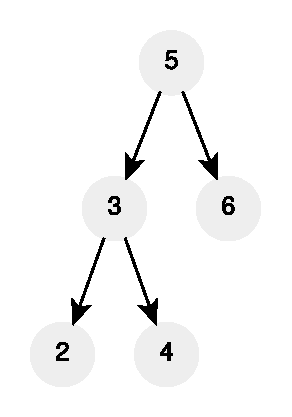
\includegraphics[width=\textwidth]{sources/smallest_range/images/example1} \caption[Sample short
%   cpation]{Sample Caption}. \label{fig:smallest_range:example1} \end{figure}

\chapter{Smallest Range \RN{1} and \RN{2}}
\label{ch:smallest_range}
\section*{Introduction}
This chapter discusses a problem and one of its variations on arrays. Both are very common interview
questions, with the former having a really easy solution, and the latter being slightly more
complex. Both variants however, can be solved by starting from the same idea and in just a handful
of lines of code.

\section{Problem statement}
\begin{exercise}
\label{example:smallest_range:exercice1}
Write a function that given given an array of integers $I$ and an integer $K \geq 0$ returns the
smallest possible difference between the smallest and largest value in $I$ after you have added to
each of the elements $-K \leq p \leq K$.

	%example1
	\begin{example}
		\label{example:smallest_range:example1}
		\hfill \\
		Given $I = \{3,5,1,7,8\}$ and $K=4$ the function returns $0$. You can add to $I$ the
		followings values: $\{1,-1,3,-3,-4\}$. The modified array becomes: $B=\{4,4,4,4,4\}$. 
	\end{example}

	%example2
	\begin{example}
		\label{example:smallest_range:example2}
		\hfill \\
		Given $I = \{1,9,4\}$ and $K=2$ the function returns $4$.
	\end{example}
\end{exercise}

\section{Clarification Questions}

\begin{QandA}
	\item Can you add $p$ multiple times to an element of $I$?
	\begin{answered}
		\textit{No, you can only add $p$ once to each element of $I$.}
	\end{answered}	
\end{QandA}

\section{Discussion}
\label{smallest_range:sec:discussion}
For this problem we are going to skip even discussing a brute-force solution\footnote{Constructing
	and returning the difference between the largest and smallest element among all of the
	$2K^{|I|}$ possible arrays you can obtain by adding any of the $2K$ between $-K$ and $K$ to each
	and every element of $I$.} because it is impractical to actually code it during an interview.
	Moreover, such a solution is conceptually very different and time complexity-wise far off from
	the one that allows us to solve this problem efficiently. So let's jump directly into the core
	of a good solution.

The problem is asking us to minimize the difference between the largest value ($M$) and the smallest
value ($m$) of $I$ after we have processed it by adding to each and every of its element a value in
the range $[-K,+K]$. Let's call $B$ this post-processed version of $I$. We know that if $K$ is large
enough\footnote{When I say "large enough" I really mean that $(M-K) - (m+K) = M-m-2K \leq 0$.} so
that we can modify $M$ and $m$ to be the same value by subtracting from $M$ and adding to $m$, then
we make all the elements of $I$ equal, thus reducing the difference between $I$'s smallest and the
largest element to zero (see Figure \ref{fig:smallest_range:explanation2}). This is possible because
$M-m$ is the  largest difference in $I$ and if we can effectively close their gap to $0$ then we can
do the same with any other difference between any pair of elements of $I$. On the other hand, if $K$
is not large enough\footnote{When $(M-m) > 2K$.} , then all we know is that we can reduce the
difference between $m$ and $M$ to $d=(M-K)-(m+K)$. Notice that in this case $d > 0$  (see Figure
\ref{fig:smallest_range:explanation1}). Moreover, similarly to what we have discussed above, because
the difference between any other pair of elements of $I$ is smaller or equal than ($M-m$), we also
know that their differences can be made at least equal or smaller than $d$.


\begin{figure}
	\vspace*{-0.5in}
	\centering
	\begin{subfigure}[t]{0.90\textwidth}
		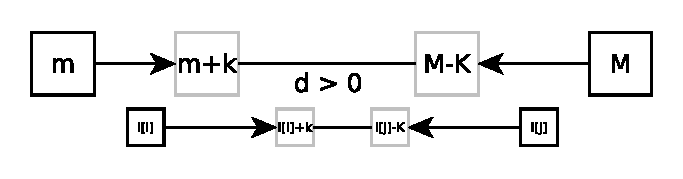
\includegraphics[width=\textwidth]{sources/smallest_range/images/explanation1} 
		\caption{$m$ and $M$ are the smallest and largest element of $I$, respectively. You can
		bring them closer together by adding $K$ to $m$ and subtracting $K$ to $M$. $d$ is the
		difference between these two new values. $d$ will always be larger than any other difference
		you can obtain the same way. You can see that any other pair $(I[i], I[j])$ will have
		smaller difference because they are closer together to begin with.}
		\label{fig:smallest_range:explanation1} 
	 \end{subfigure}
	\medskip
	\begin{subfigure}[t]{0.90\textwidth}
		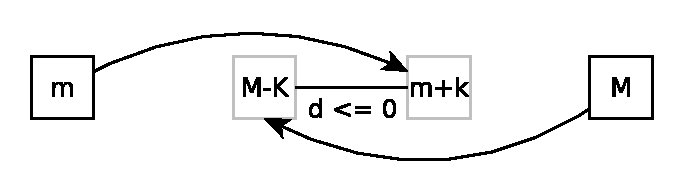
\includegraphics[width=\textwidth]{sources/smallest_range/images/explanation2} 
		\caption{$m$ and $M$ are the smallest and largest element of $I$, respectively. If we  add
		$K$ to $m$ and subtract $K$ to $M$ then in this case $(m+K)$ will be larger than $(M-K)$.
		This means that we can add to $m$ and subtract to $M$ a number $p \leq K$ such that $m+p =
		M-p$. Because any other number in $I$ is larger than $m$ and smaller than $M$ we can do the
		same with them, so that we bring all the elements to the same value.}
		\label{fig:smallest_range:explanation2} 
	 \end{subfigure}
	 \medskip
	 \label{}
	 \caption{}
\end{figure}
Therefore in order to solve this problem we only have to look at $M$ and $m$ and calculate
$d=(M-K)-(m+K)$. If $d \leq 0$ then it means that we can make all the elements of $I$ equal and the
function should return $0$, otherwise we can safely return $d$ as an answer.

You can find an implementation of this idea in Listing \ref{list:smallest_range:solution1} which has
$O(|I|)$ time and $O(1)$ space complexity. The
\inline{std::minmax_element}\footnote{\url{https://en.cppreference.com/w/cpp/algorithm/minmax_element}}
function  returns a pair of iterators pointing to the minimum and maximum element of the input
range, respectively.
\lstinputlisting[language=c++, caption={Solution to the \textit{smallest range} problem.},label=list:smallest_range:solution1]{sources/smallest_range/smallest_range_solution1.cpp}


\section{Common Variations}
%https://leetcode.com/discuss/explore/december-leetcoding-challenge/980929/Smallest-Range-II%3A-Python-5LoC-with-Pictorial-Explanation-O(n-log-n)-Time-Memory-Beats-99.40/796292
\subsection{Smallest range \RN{2} } This variant is almost identical to the main problem of this
chapter (see Exercise \ref{example:smallest_range:exercice1}) except that this time we are only
allowed to add either $-K$ or $+K$ (and not any number in the range $[-K,K$) to each and every
element of the input array $I$. As we shall see, this complicates things quite a bit, but,
nevertheless, the core solution strategy remains the same. 

\begin{exercise}
	\label{example:smallest_range:variation1:exercice1}
	Write a function that given given an array of integers $I$ and an integer $K$ returns the
	smallest possible difference between the smallest and largest value in $I$ after you have added
	to each of the elements either $-K$ or $K$.
	
		%example1
		\begin{example}
			\label{example:smallest_range:variation1:example1}
			\hfill \\
			Given $I = \{3,5,1,7,8\}$ and $K=2$ the function returns $3$. You can modify add to
			$I$ the followings values $\{2,-2,2,-2,-2\}$. The modified array finally becomes:
			$I'=\{5,3,3,5,6\}$. 
		\end{example}
	
		%example2
		\begin{example}
			\label{example:smallest_range:variation1:example2}
			\hfill \\
			Given $I = \{1,9,4\}$ and $K=3$ the function returns $3$.
		\end{example}
	
	\end{exercise}

	\begin{figure}
		\centering
		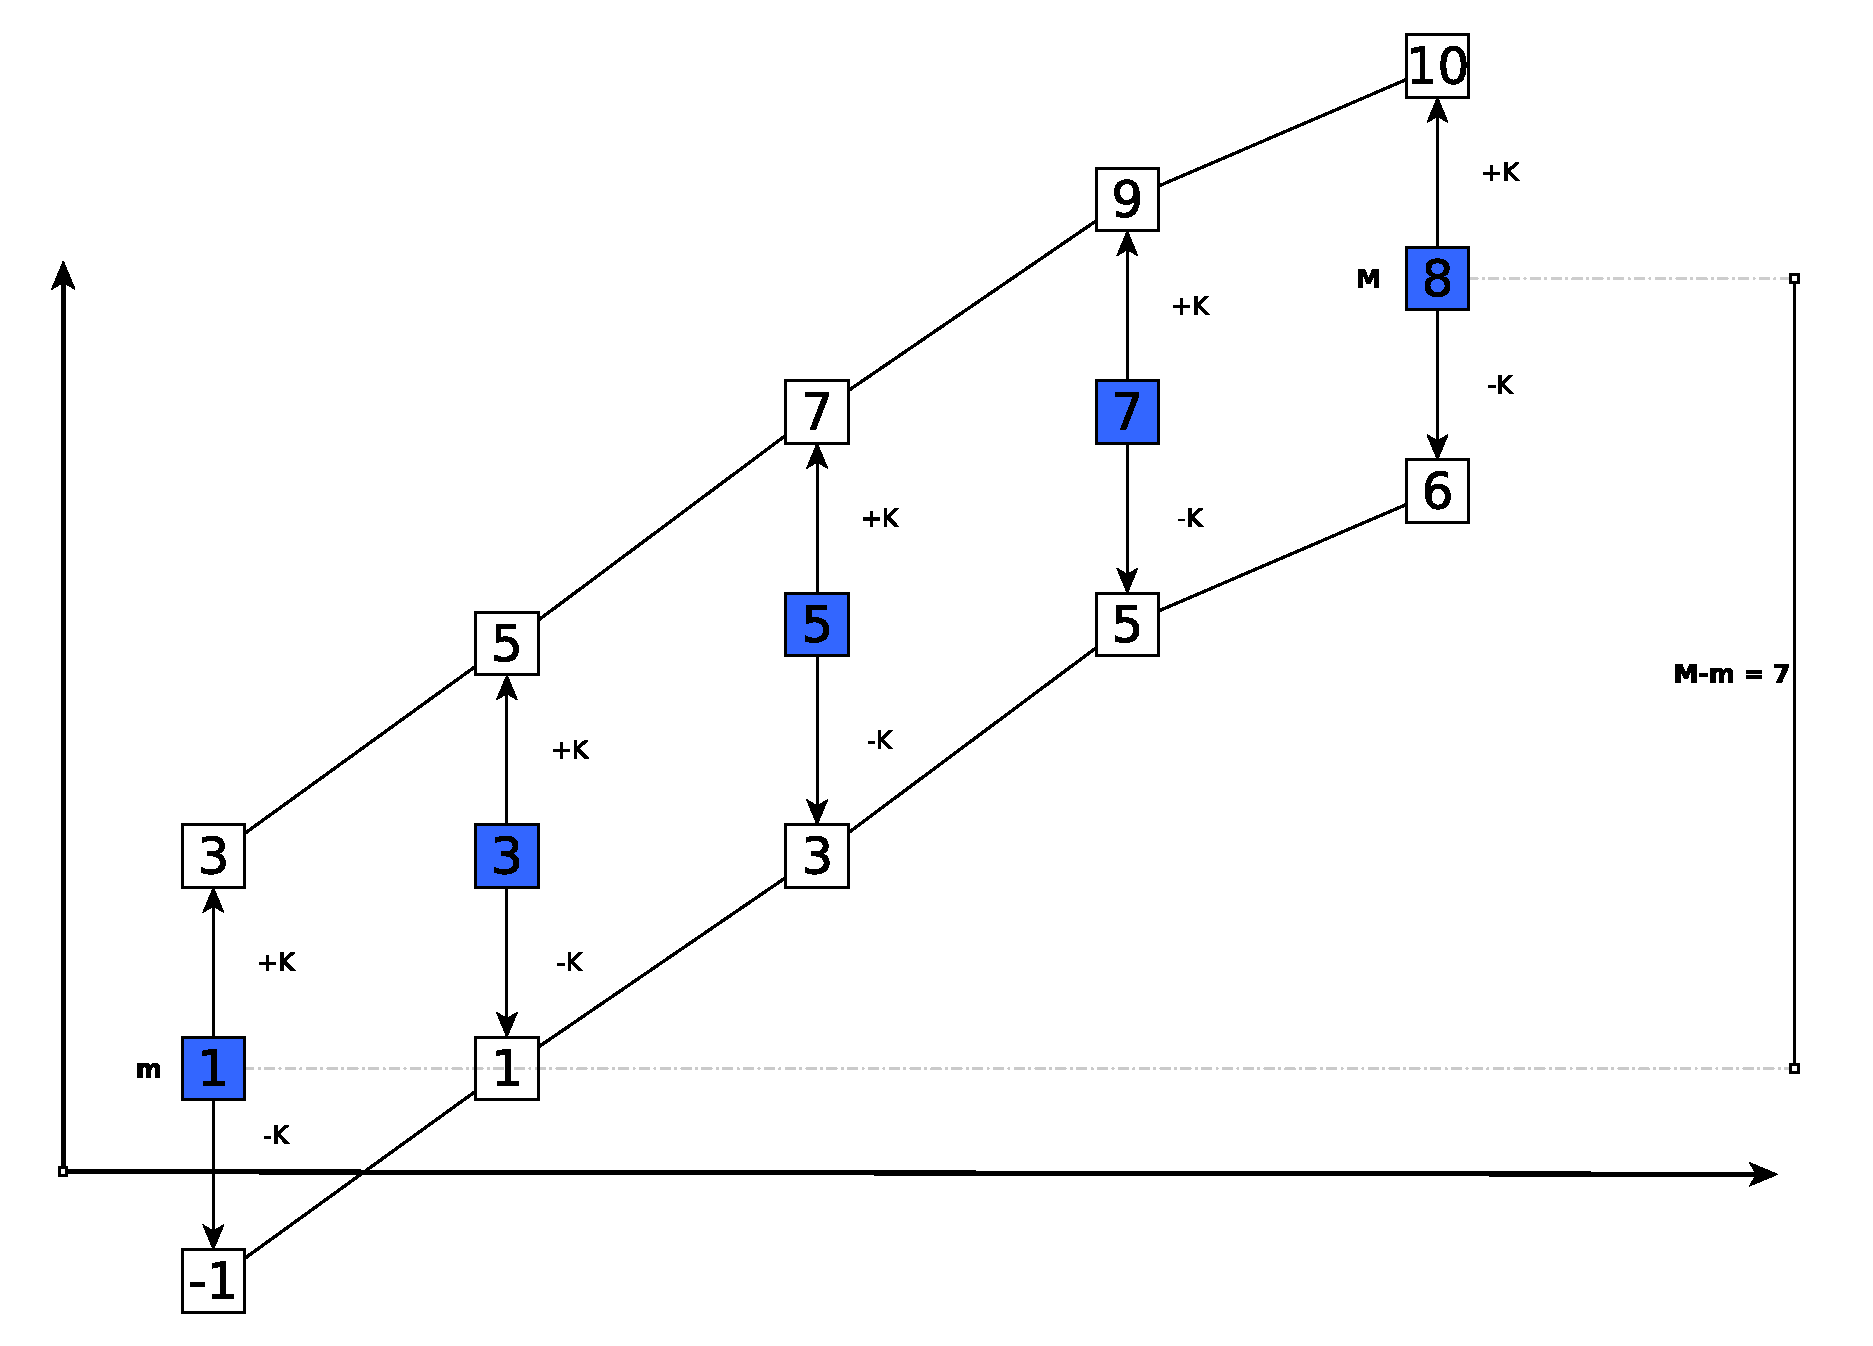
\includegraphics[width=1\linewidth]{sources/smallest_range/images/bars}
		\caption{This figure is visual representation of the Example \ref{example:smallest_range:variation1:example1}
		where the highlighted boxes represent the input values, the white boxes on the higher part of
		the picture represent the values we can get by adding $K$ to the corresponding element and the
		white boxes in the bottom part of the picture shows the values we can get by subtracting $K$ to
		them.}
		\label{fig:smallest_range:bars_full}
	\end{figure}

\section{Discussion}
\label{smallest_range:sec:discussion}
Let's start by noticing that the solution to this problem is always smaller or equal than the
difference between the largest ($M)$ and smaller  $(m)$ elements of $I$. This is the case because in
the worst case we can either add or subtract $K$ to all of the elements of $I$ and therefore
preserve the relative difference between all the elements of $I$ (including $M$ and $m$). We have
this case when $(M-m) \leq K$ because subtracting and adding $K$ to $M$ and $m$, respectively, would
eventually lead to a larger or equal difference\footnote{The intuition behind this is that adding
$K$ to $m$ would yield $m' = m+K$ which is greater or equal than $M$. Similarly, subtracting $K$ to
$M$ would yield $M' = M-K$ which is smaller or equal than $m$. The gap between $m'$ and $M'$ is
larger or equal than the gap between $m$ and $M$. When $(M-m) < K$ then we can express $K$ in terms
of $M-m$ as follows: $K = M-m + x$ where $x \geq 0$. Therefore by adding $K$ to $m$ and subtracting
$K$ to $M$ we get: $|(M-K) - (m-K)| = |(M-(M-m + x)) - (m + (M-m + x))| = |(m-x) - (M+x)|$ which is
at least as large as $M-m$.

For instance given $I = \{1,2,6,8\}$ and $K = 10 > (8-1) = 7$ if we add $10$ to the smallest element
of $I$ and substract $10$ to its largest, we end up with: $1+10 = 11$ and $8-10=-2$. The difference
between these two new values is $11-(-2) = 13$ which is definitely larger than the difference
between $1$ and $8$.}.

When $(M-m) > K$ then what we can do is to choose one element at index $j$ as a sort of pivot point
and add $K$ to all the elements smaller or equal than $I_j$ and subtract $K$ to all of the elements
of $I$ greater than $I_j$. The new gap depends on the new smallest ($m'$) and largest elements
($M'$). Given $p$ is the smallest element larger than $I_j$ then, $M'$ is the largest among $I_j+K$
and $M-K$ while $m'$ is the smallest among $p - K$ and $m+K$. Therefore for a given $j$ we calculate
the maximum gap as $d_j = M'-m'$. The final answer is the smallest of these gaps calculated for each
of index of $I$.

This approach relies on being able to quickly identify elements that are smaller or greater than a
given value. If the array is sorted this can be achieved quite efficiently. In-fact is $I$ is sorted
then for a given $j$ all the elements that are smaller than $I_j$ appear at indices smaller than $j$
and, similarly, all the elements that are larger appear at indices larger than $j$. Therefore, if
$I$ is sorted then $m'$ is the smallest among $I_{j+1}-K$ and $I_0 +K$ and $M'$ is the largest among
$I_j+K$ and $I_{|I|-1}-K$.


We can use these observation to derive the following algorithm:
\begin{enumerate}
	\item sort the input array $I$,
	\item for each $j = 0 \ldots |I|-1$ calculate $d_j = \max{(I_j+K,I_{|I|-1}-K)} -
	\min{(I_{j+1}-K, I_0 +K)}$,
	\item return the smallest $d_j$.
\end{enumerate}
An execution of this algorithm for the Example \ref{example:smallest_range:variation1:example1} is
shown in the Figure \ref{fig:smallest_range:bars_execution}. The initial input is shown in Figure
\ref{fig:smallest_range:bars_full} where the smallest and greatest value are $m=1$ and $M=8$,
respectively. The only way for their gap to become smaller is for $M$ to be decreased and $m$ to be
increased by $K$. Figure \ref{fig:smallest_range:bars2} shows how $I$ would look like if we would
add $K$ to all the elements smaller or equal than $j=0$ and subtract $K$ to the others. The
highlighted boxes show the new array values while the white boxes show the original values. Notice
that the gap between the new minimum ($1$, obtained by subtracting $2$ from the original element
with value $3$) and the new maximum element ($6$, obtained by subtracting $2$ from $8$) is now
$6-3=3$. Similarly Figure \ref{fig:smallest_range:bars3} shows the resulting array for $j=3$. The
new array minimum and maximum values are now $3$ and $6$, respectively. When $j=2$ or $j=3$, as we
can see in Figures \ref{fig:smallest_range:bars4} and \ref{fig:smallest_range:bars5} the gap
increases w.r.t. to the case where $j=1$. Finally Figure \ref{fig:smallest_range:bars6} shows the
case where all the new elements are obtained by adding $K$. This scenario leaves the relative
distance between the elements unchanged w.r.t. to the original values and therefore not surprisingly
the gap between the smallest and largest element is $7$ (like in Figure
\ref{fig:smallest_range:bars_full}).


Listing \ref{list:smallest_range:solution2} shows an implementation of this idea. Notice that, in
the code, $m'$ is \inline{m_new} and $M'$ is \inline{M_new}.
\lstinputlisting[language=c++, caption={Solution to the \textit{smallest range} problem using sorting.},label=list:smallest_range:solution2]{sources/smallest_range/smallest_range_solution2.cpp}

\begin{figure}
	\centering
	\vspace{-0.5in}
	
	\begin{subfigure}[t]{0.99\textwidth}
			\centering
			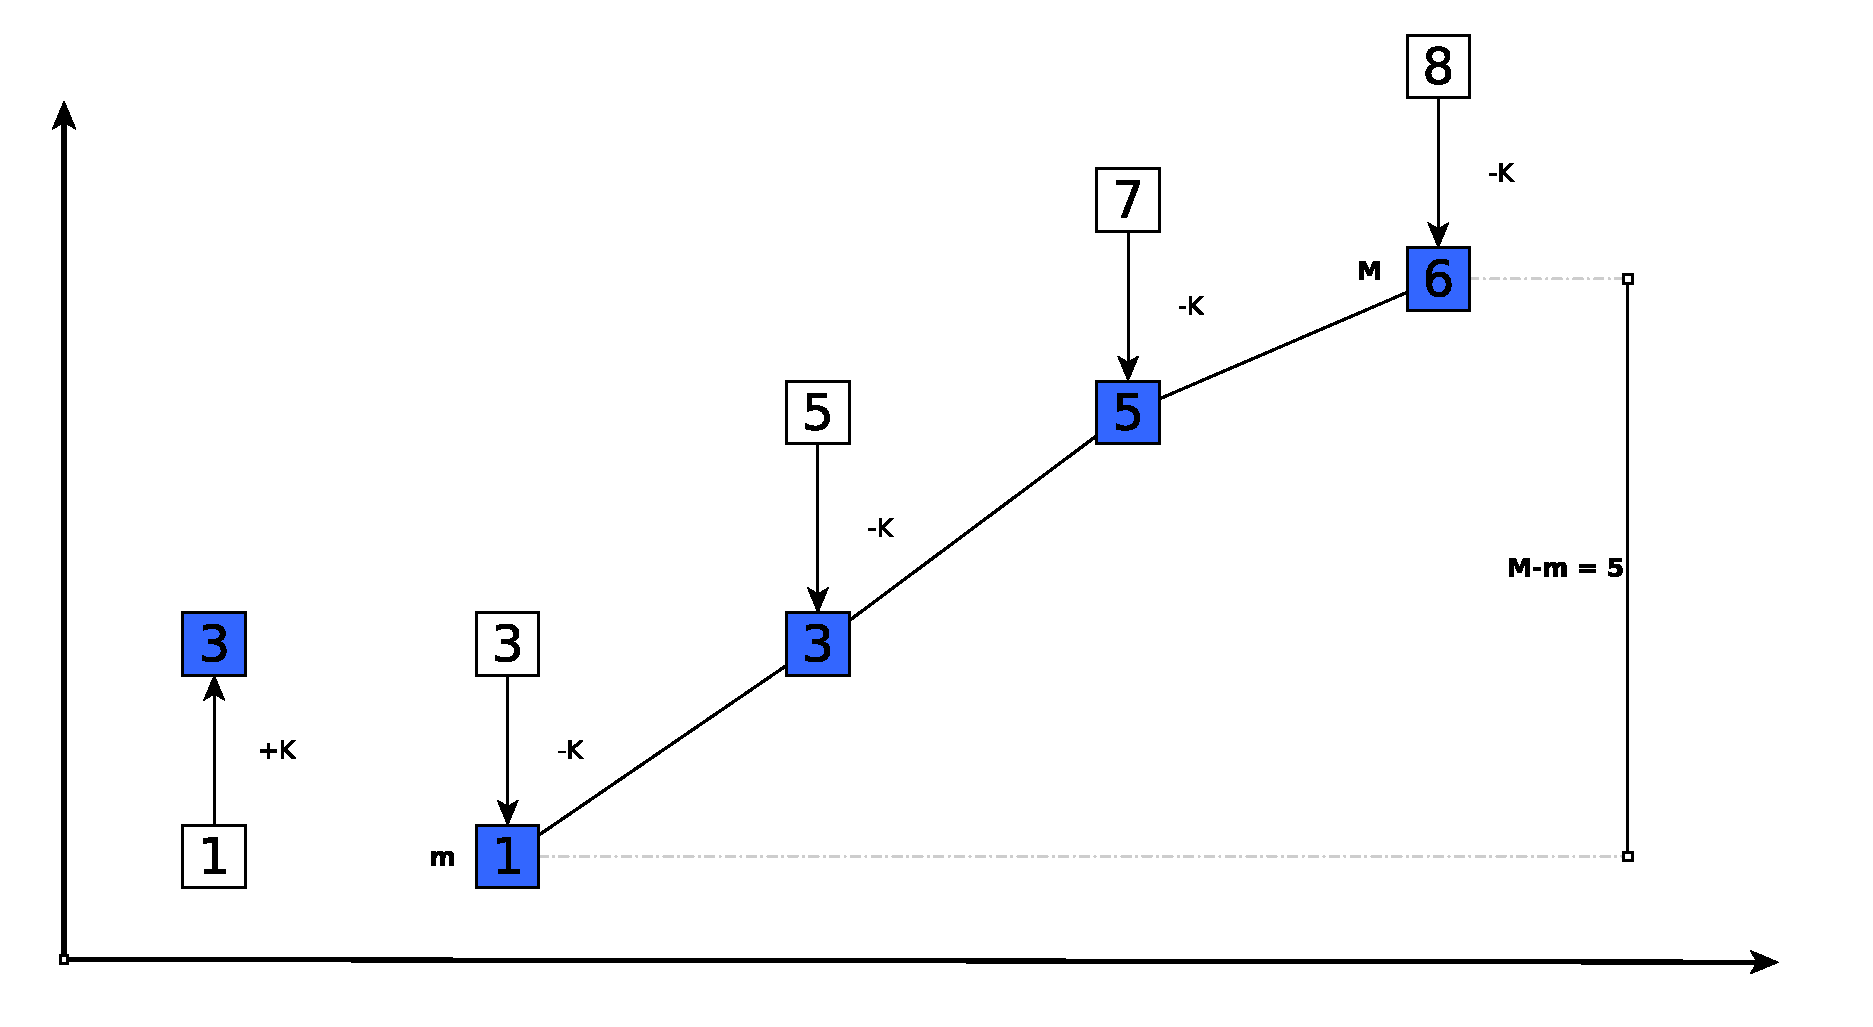
\includegraphics[width=1\linewidth]{sources/smallest_range/images/bars2}
			\caption{$j=0$}
			\label{fig:smallest_range:bars2}
	\end{subfigure}
	
	\begin{subfigure}[t]{0.99\textwidth}
		\centering
		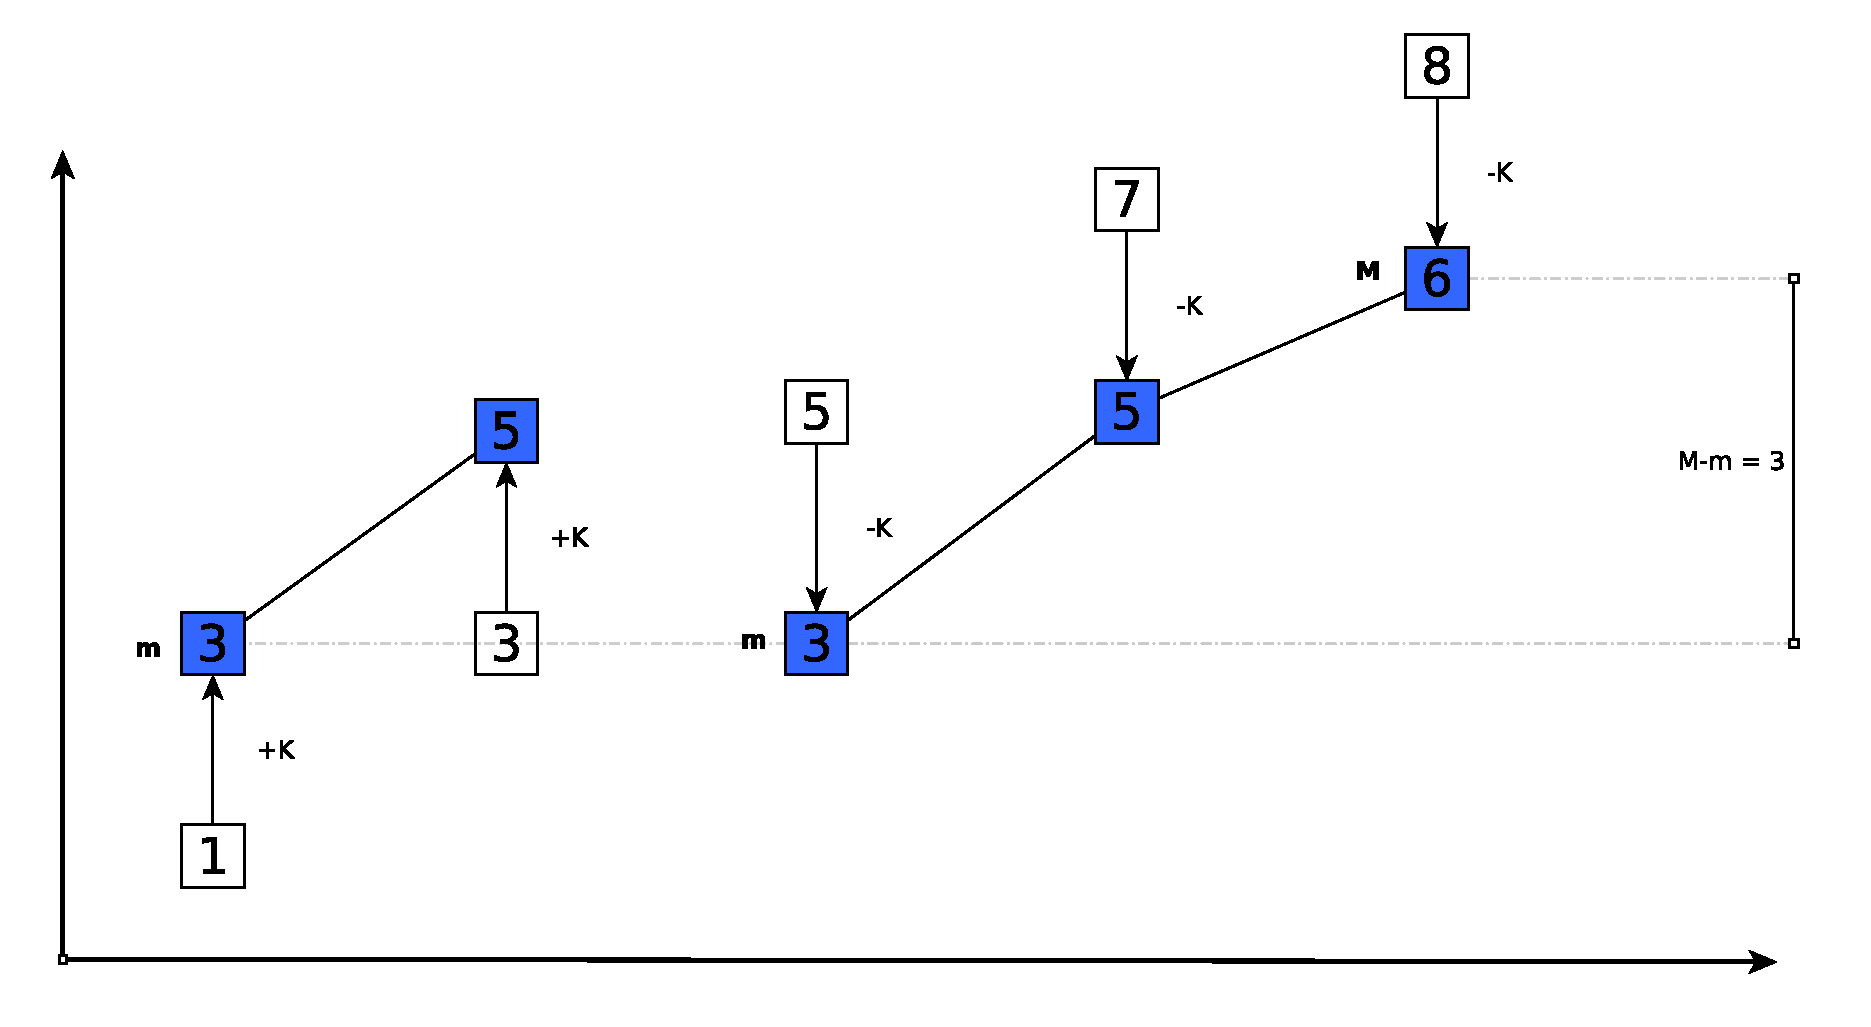
\includegraphics[width=1\linewidth]{sources/smallest_range/images/bars3}
		\caption{$j=1$}
		\label{fig:smallest_range:bars3}
	\end{subfigure}

	
	\medskip
	\begin{subfigure}[t]{0.99\textwidth}
		\centering
		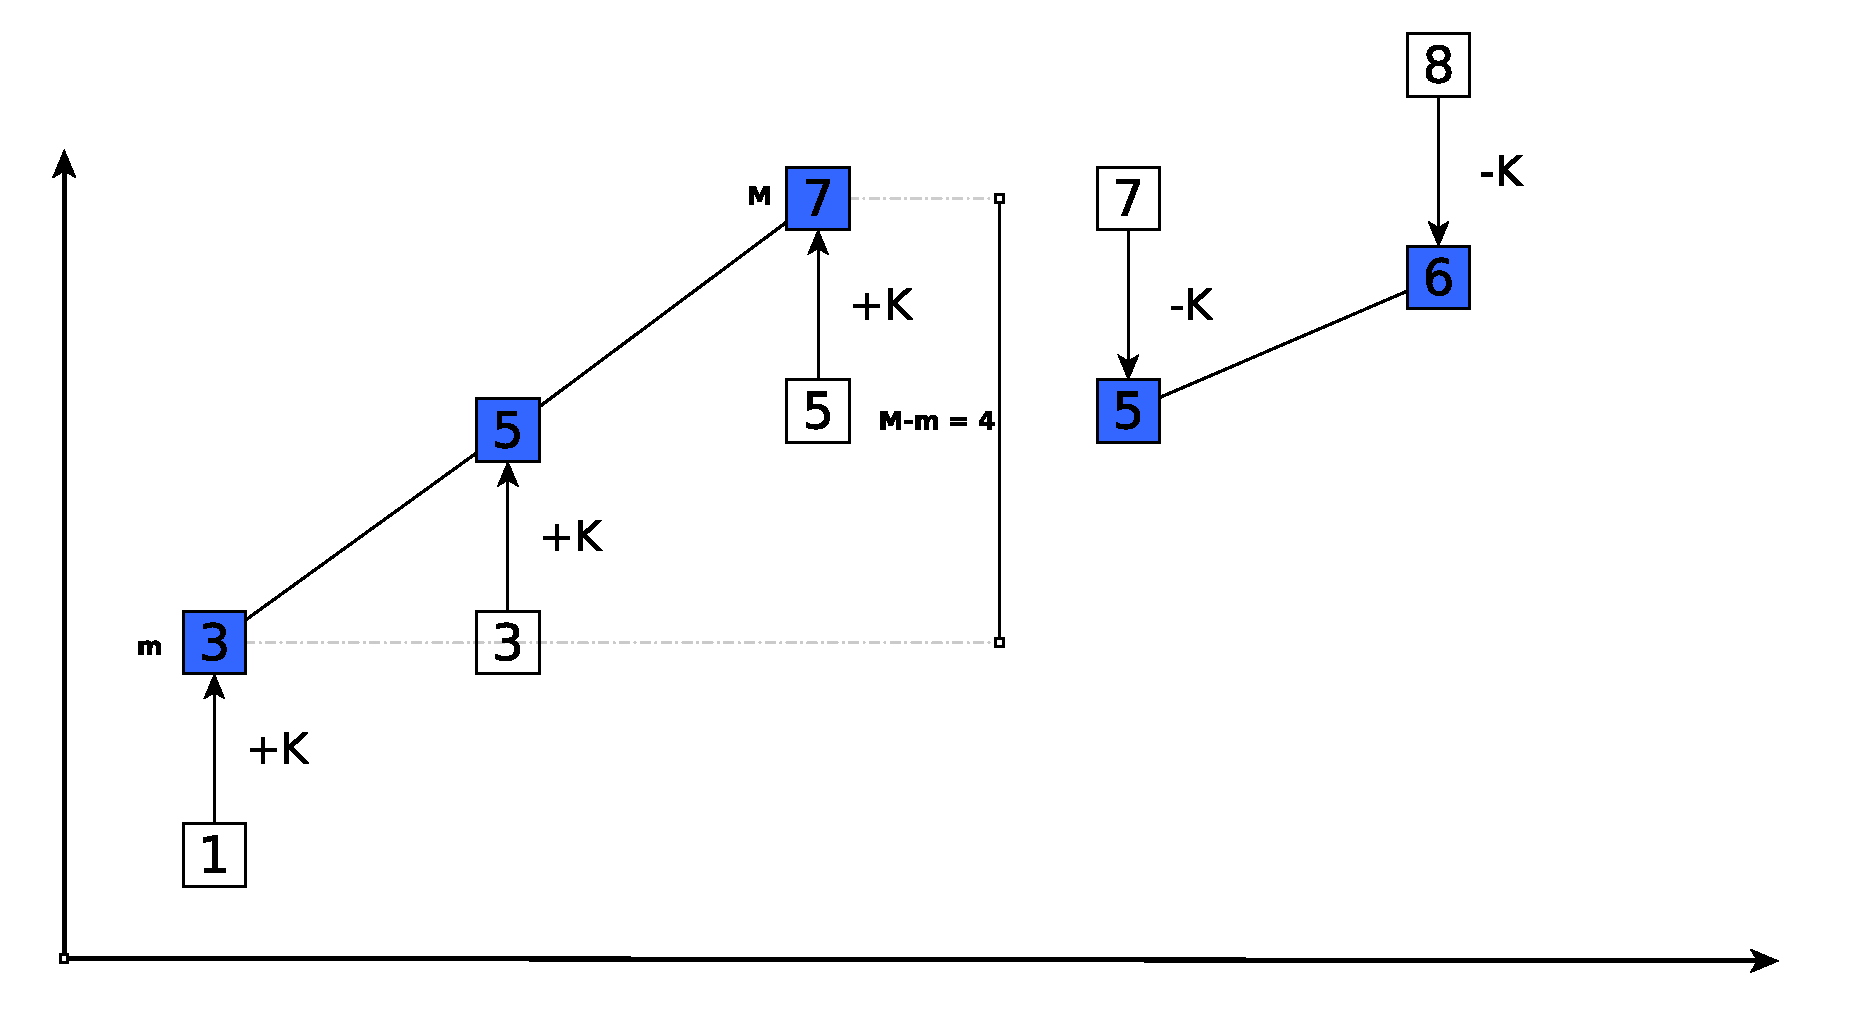
\includegraphics[width=1\linewidth]{sources/smallest_range/images/bars4}
		\subcaption{$j=1$}
		\label{fig:smallest_range:bars4}
	\end{subfigure}
\end{figure}


\begin{figure}\ContinuedFloat
	\begin{subfigure}[t]{0.99\textwidth}
		\centering
		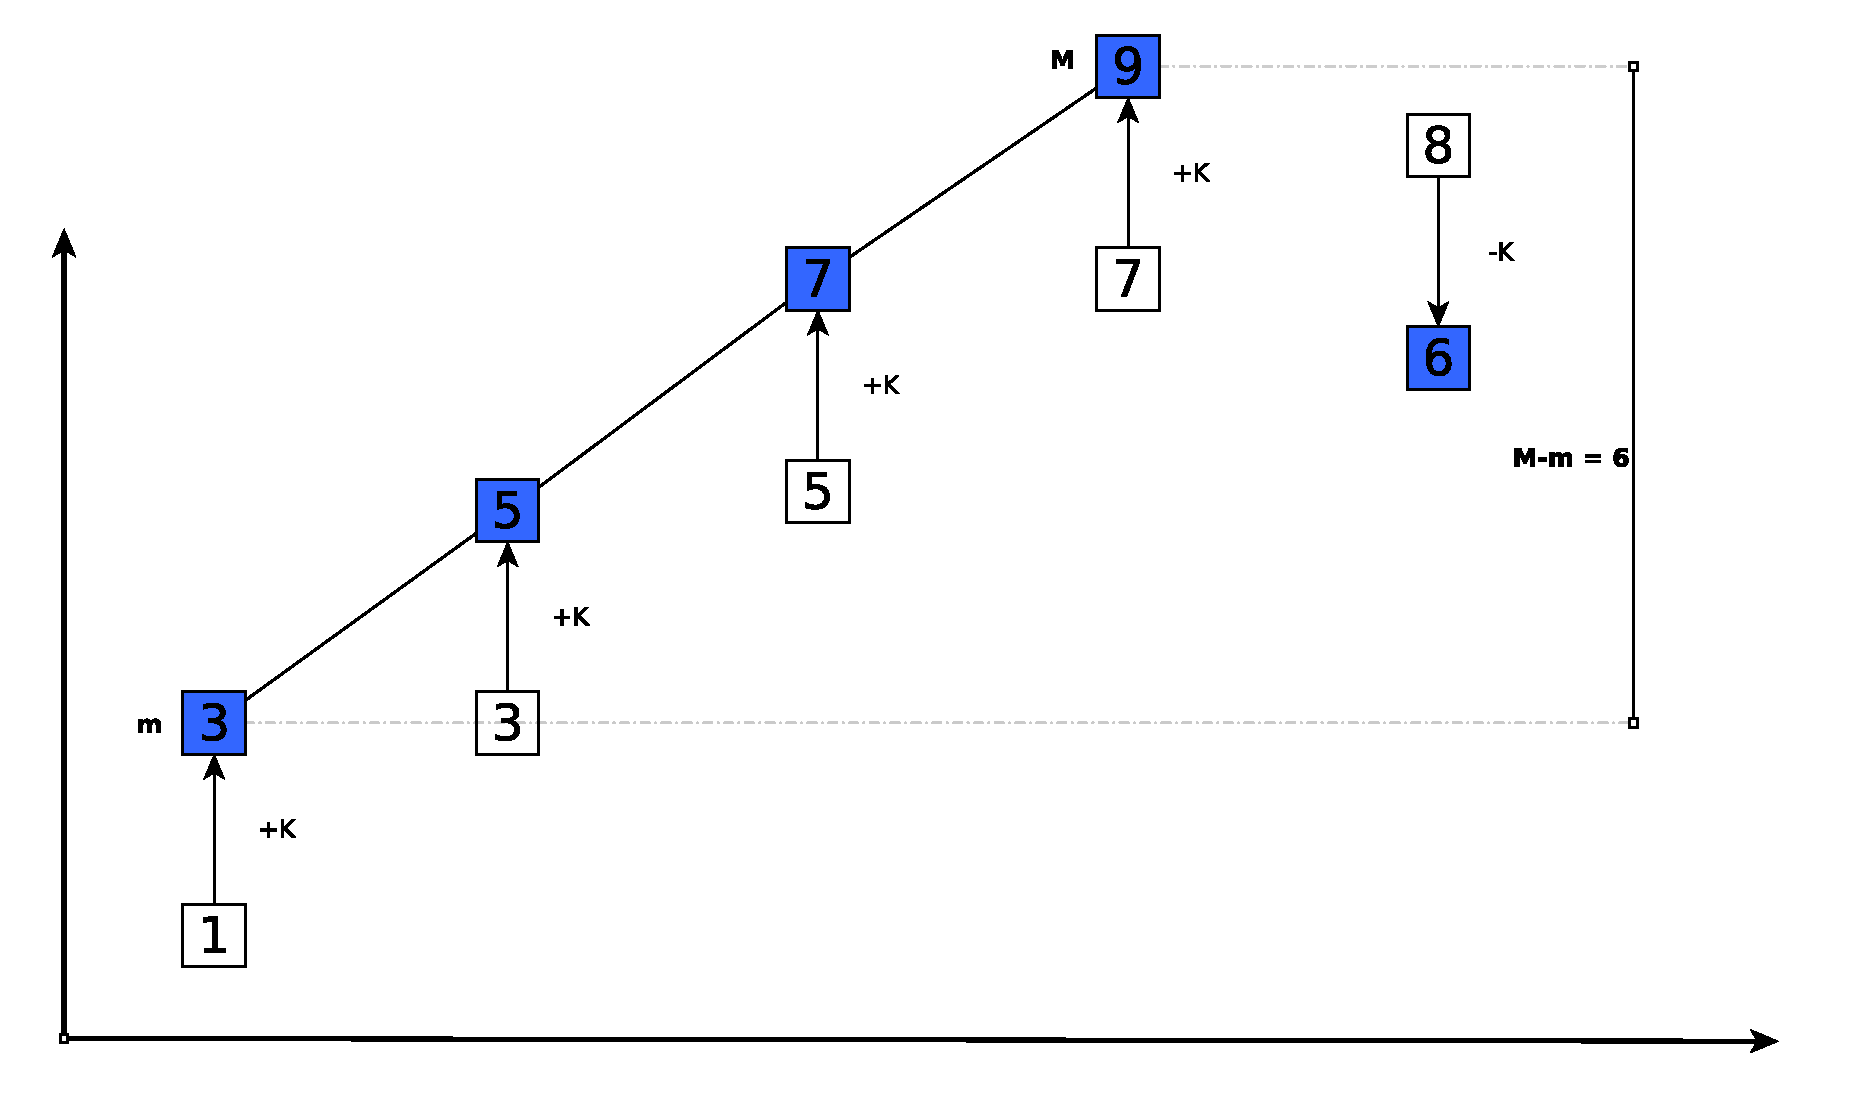
\includegraphics[width=1\linewidth]{sources/smallest_range/images/bars5}
		\caption{$j=1$}
		\label{fig:smallest_range:bars5}
	\end{subfigure}

	\medskip
	\begin{subfigure}[t]{0.99\textwidth}
		\centering
		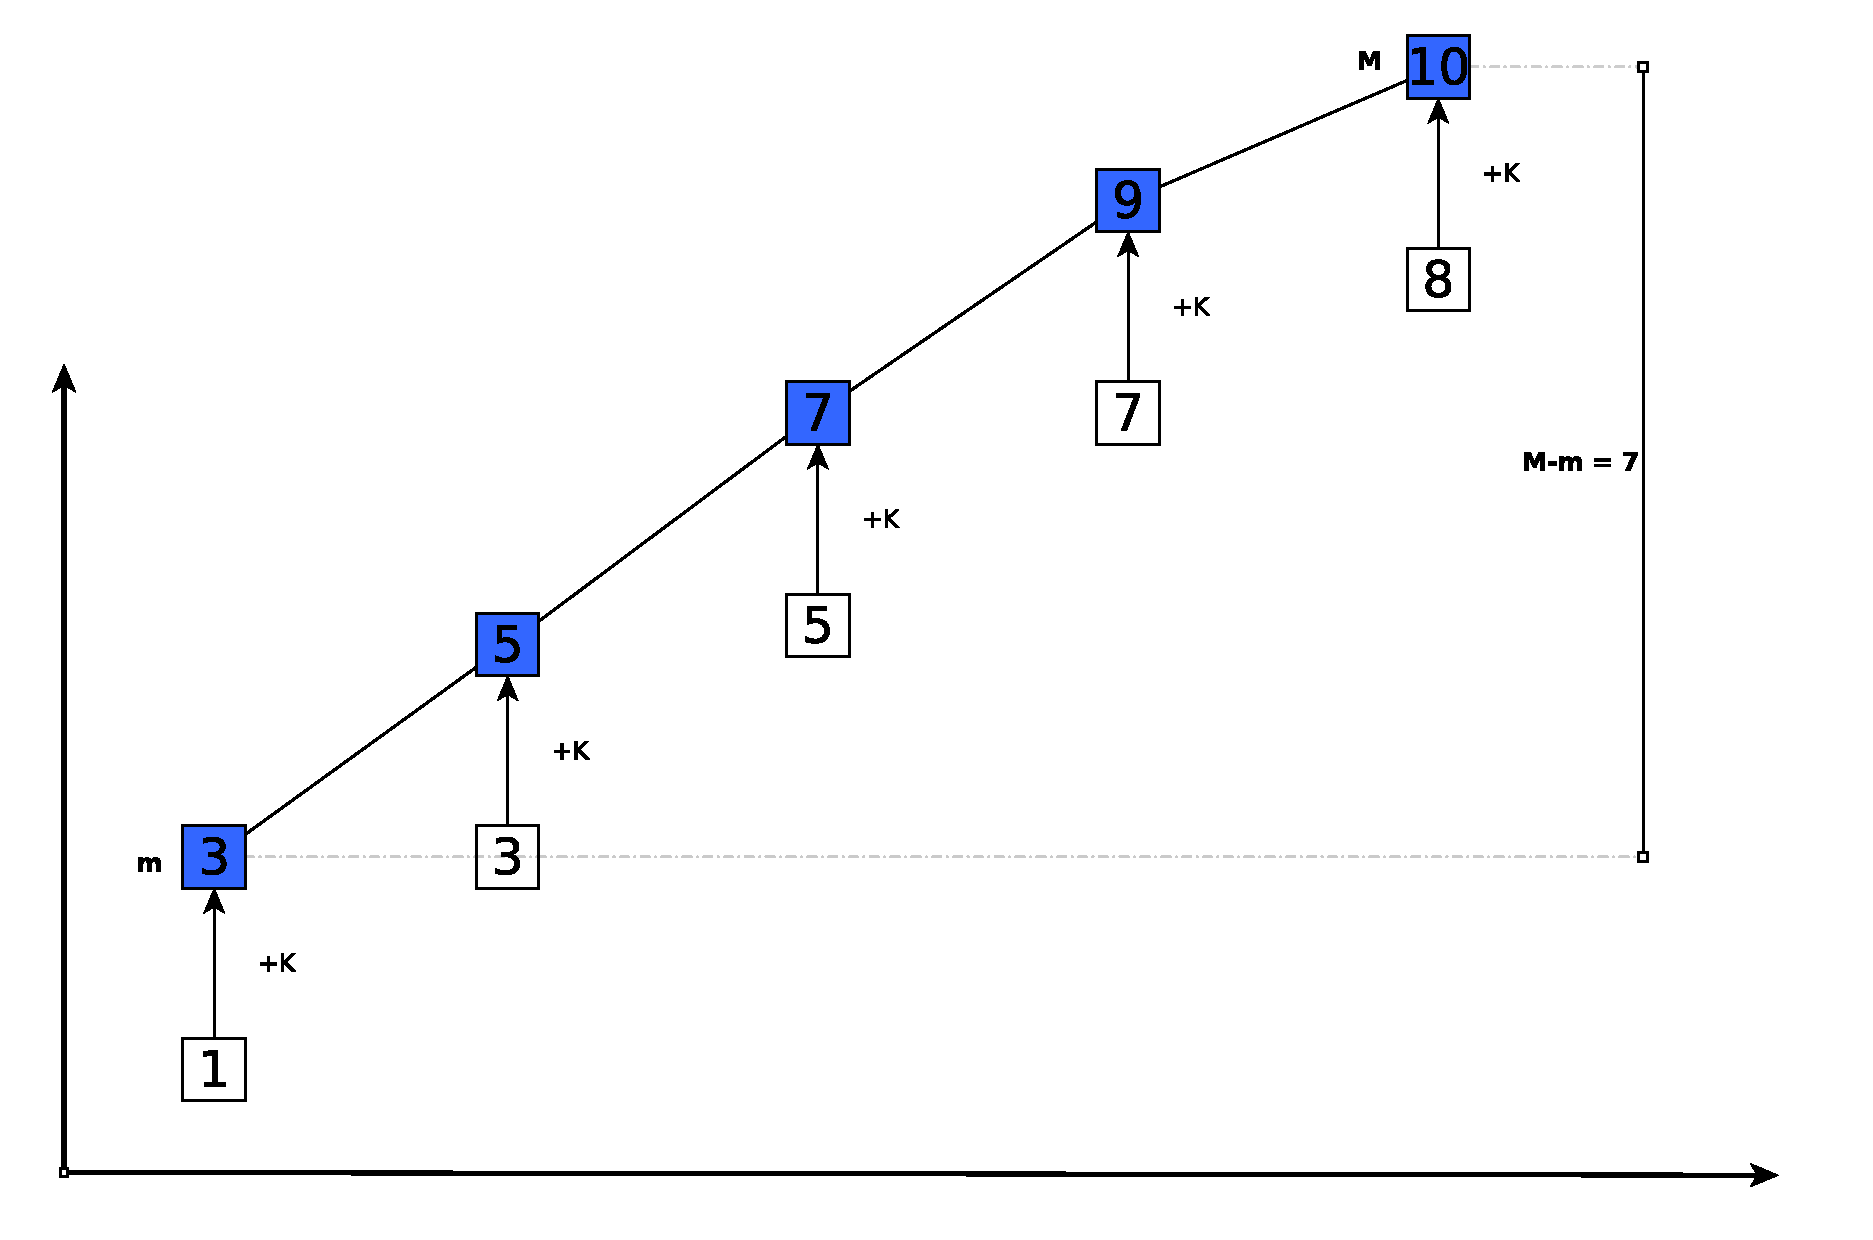
\includegraphics[width=1\linewidth]{sources/smallest_range/images/bars6}
		\caption{$j=1$}
		\label{fig:smallest_range:bars6}
	\end{subfigure}

	\caption{Execution of the algorithm presented in Section \ref{smallest_range:sec:discussion}
	for $j=0$ (Figure \ref{fig:smallest_range:bars2}),  $j=1$ (Figure \ref{fig:smallest_range:bars3}),
	$j=2$ (Figure \ref{fig:smallest_range:bars4}), $j=5$ (Figure \ref{fig:smallest_range:bars4}) 
	and $j=5$ (Figure \ref{fig:smallest_range:bars5}).
	The highlighted boxes contains the values obtained from the original elements
	shown in the white boxes.}
	\label{fig:smallest_range:bars_execution}
\end{figure}